%\chapter*{TP 14 \\ 
%Création et Parcours d'un labyrinthe -- \ifprof Corrigé \else Sujet \fi}
%\addcontentsline{toc}{section}{TP 14 : 
%Création et Parcours d'un labyrinthe -- \ifprof Corrigé \else Sujet \fi}
%
%\iflivret \stepcounter{cptApplication} \else
%\ifprof  \stepcounter{cptApplication} \else \fi
%\fi


\begin{marginfigure}
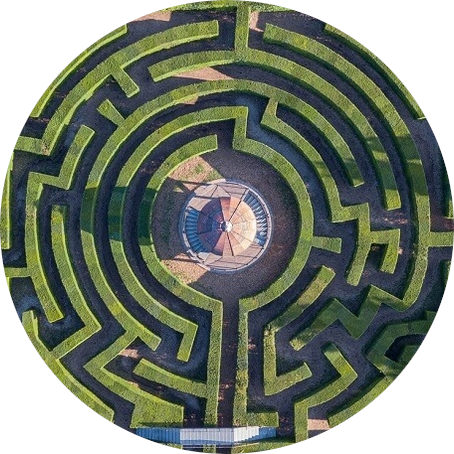
\includegraphics[width=\linewidth]{fig_00.png}
\end{marginfigure}

\marginnote{Inspirations : 
\href{https://www.lama.univ-savoie.fr/mediawiki/index.php/Génération_et_résolution_de_labyrinthes}{Génération et résolution de labyrinthes}
 et  
\url{https://cpge-itc.github.io/itc1/5_graph/3_traversal/labyrinth/}}




\subsection*{Génération d'une grille}

Soit une grille rectangulaire $n\times p$ constituée de $n$ colonnes et de $p$ lignes contenant toutes les arêtes possibles. On modélise cette grille par un graphe dont l'ensemble des sommets est donné par les couples $(i,j)$ tels que $i\in\llbracket 0,n \llbracket $ et $j\in\llbracket 0,p \llbracket $. Les voisins d'un sommet $(i,j)$ sont ceux situés en haut, en bas, à droite et à gauche s'ils existent (par exemple, le sommet $(0,0)$ a comme voisin les sommets $(0,1)$ et $(1,0)$).



\begin{figure}[!h]
\centering
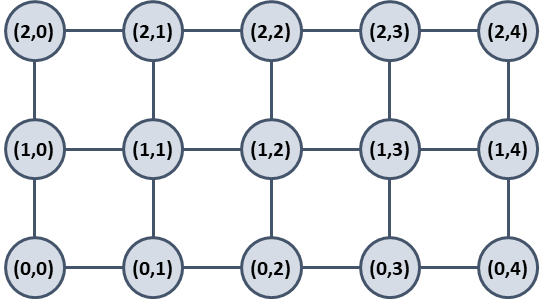
\includegraphics[width=12cm]{fig_01}
\caption{Grille (5,3) et grille (2,2)}
\end{figure}

Le graphe est implémenté par un dictionnaire d'adjacence où les clés sont les tuples, coordonnées d'un sommet. La valeur associée est une liste des sommets voisins. 



\question{Écrire la fonction \cde{creer\_graphe(n:int, p:int) -> \{\}} permettant de créer le graphe d'une grille de \lstinline{n} colonnes et \lstinline{p} lignes.}
\begin{exemple}
La grille $ 2 \times 2$ sera modélisée par le graphe suivant :
\end{exemple}

\begin{lstlisting}
>>> G2 =  creer_graphe(2,2)
>>> G2
        {(0, 0): [(1, 0), (0, 1)],
        (1, 0): [(1, 1), (0, 0)],
        (0, 1): [(1, 1), (0, 0)],
        (1, 1): [(0, 1), (1, 0)]}
\end{lstlisting}

On souhaite afficher ce graphe en utilisant \lstinline{matplotlib}. Pour cela, on va commencer par tracer chacune des arêtes puis chacun des sommets. 

\question{Écrire la fonction \lstinline{get_sommets(G:dict) -> (list,list)} renvoyant deux listes \lstinline{les_x} et \lstinline{les_y} contenant respectivement les abscisses des sommets et les ordonnées des sommets.}
\begin{exemple}
Dans l'exemple qui suit, les coordonnées de sommets peuvent être dans un ordre différent. 

\end{exemple}

\begin{lstlisting}
>>> les_sx, les_sy = get_sommets(G2)
>>> les_sx, les_sy
        ([0, 1, 0, 1], [0, 0, 1, 1])
\end{lstlisting}

\question{Écrire la fonction \cde{trace\_sommets(G:\{\}) -> None} qui affiche les sommets en utilisant un point rouge (\cde{`r.`}) ou cercle rouge (\cde{`ro`}).}

\question{Écrire la fonction \cde{get\_aretes(G:\{\}) -> []} renvoyant la liste des arêtes du graphe sous la forme d'une liste de listes de tuples. Une arête est donc une liste de sommets où les sommets sont des tuples. Les arêtes ne devront être présentes qu'une fois. }

\begin{exemple}
Dans l'exemple qui suit, l'ordre des arêtes peut être dans un ordre différent. Pour une arête donnée, les sommets peuvent aussi être dans un ordre différent.

\end{exemple}

\begin{lstlisting}
>>> get_aretes(G2)
        [((0, 0), (1, 0)), ((0, 0), (0, 1)), ((1, 0), (1, 1)), ((0, 1), (1, 1))]
\end{lstlisting}


\question{Écrire la fonction \cde{trace\_aretes(G:\{\}) -> None} qui affiche les arêtes en utilisant un trait bleu. Exemple : pour tracer l'arête [(0,2),(1,2)], il faut utiliser l'instruction \lstinline{plt.plot([0,1],[2,2],'b')}.}

\begin{marginfigure}
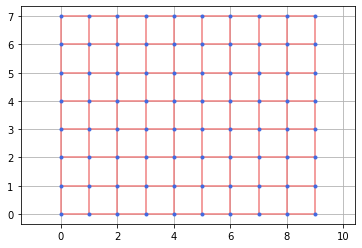
\includegraphics[width=\linewidth]{grille_10_8}
\caption{Grille 10 colonnes 8 lignes}
\end{marginfigure}

\question{Écrire la fonction \cde{trace\_graphe(G:\{\}) -> None} qui permet de tracer les sommets au dessus des arêtes.}





\subsection*{Génération d'un labyrinthe}

Dans notre cas, résoudre le labyrinthe consiste en partir du sommet de départ \lstinline{(0,0)} (sommet en bas à gauche, par exemple) et à se déplacer sur les arêtes dans le but d'atteindre le sommet en haut à droite. 
Pour générer un labyrinthe, nous allons réaliser un parcours de la grille \lstinline{G} (en largeur ou en profondeur). Le labyrinthe sera lui-même un graphe noté \lstinline{L}. À chaque fois qu'on \textbf{empilera ou enfilera} un \textbf{sommet non visité}, on ajoutera une arête entre entre ce sommet et le sommet père à \lstinline{L}. 




\question{Écrire la fonction \cde{ajouter\_arete(G:\{\}, s1:tuple, s2:tuple) -> None} qui permet d'ajouter l'arête \lstinline{([s1,s2])} au graphe \lstinline{G}. \textbf{Pour ajouter une arête, il est par exemple possible de traiter les deux cas suivants : on ajoute une arête si aucun des sommets appartient au graphe, ou si le le sommet d'arrivée n'existe pas dans le graphe}. }
\begin{exemple}
On reprend le graphe noté \lstinline{G2} précédemment. 

\end{exemple}
\begin{lstlisting}
>>> ajouter_arete(G2,(1,0),(2,0))
>>> G2
        {(0, 0): [(1, 0), (0, 1)],
        (1, 0): [(1, 1), (0, 0), (2, 0)],
        (0, 1): [(1, 1), (0, 0)],
        (1, 1): [(0, 1), (1, 0)],
        (2, 0): [(1, 0)]}
\end{lstlisting}

\begin{marginfigure}[-2cm]
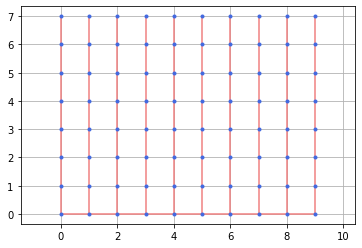
\includegraphics[width=\linewidth]{grille_10_8_largeur.png}
\caption{Labyrinthes en largeur}
\end{marginfigure}

\question{Écrire la fonction \cde{parcours\_largeur(G:\{\}, depart:tuple) -> dict} qui permet de créer un labyrinthe en largeur à partir d'un graphe \lstinline{G}. Tracer le labyrinthe obtenu. \lstinline{s} sera ici le point de départ du labyrinthe,\lstinline{(0,0)} par exemple.}




\question{Écrire la fonction \cde{parcours\_profondeur(G:\{\}, s:tuple) -> dict} qui permet de créer un labyrinthe en profondeur à partir d'un graphe \lstinline{G}. Tracer le labyrinthe obtenu.}



\begin{marginfigure}
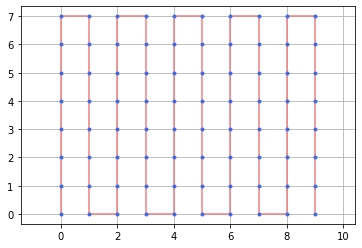
\includegraphics[width=\linewidth]{grille_10_8_profondeur.png}
\caption{Labyrinthes en profondeur}
\end{marginfigure}

Comme vous pouvez le constater, le coté aléatoire de ces labyrinthes est discutable :). Le labyrinthe que vous pourrez obtenir peut varier, notamment en fonction, de l'ordre dans lequel vous ajoutes les sommets dans le graphe dans la fonction \lstinline{creer_graphe}. 
Il est possible de mélanger une liste en utilisant le module \lstinline{random} : \lstinline{random.shuffle(voisins)} permet de mélanger la liste de tuples \lstinline{voisins}.

\begin{marginfigure}
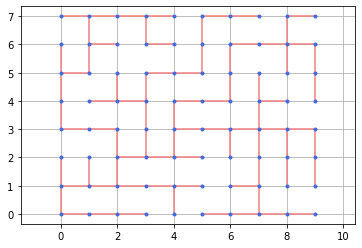
\includegraphics[width=\linewidth]{labyrinthe_10_8_profondeur.png}
\caption{Labyrinthe 10x8}
\end{marginfigure}


\question{Écrire les fonctions \cde{labyrinthe\_largeur(G:\{\}, s:tuple) -> \{\}} et \cde{labyrinthe\_profondeur(G:\{\}, s:tuple) -> \{\}} permettant de prendre cette remarque en compte. Quelle fonction permet d'obtenir un labyrinthe acceptable ?}



\subsection*{Résolution d'un labyrinthe}

Il est possible de résoudre le labyrinthe en utilisant un parcours en largeur ou un parcours en profondeur. 

\question{Écrire la fonction \cde{resolution\_largeur(G:\{\}, s:tuple) -> []} qui permet de résoudre le labyrinthe en utilisant un parcours en largeur. Cette fonction renvoie la liste des sommets permettant d'atteindre le sommet en haut à droite depuis le sommet en bas à gauche.}

\question{Afficher en trait épais noir la solution donnée par le parcours en largeur.}

\question{Répondre aux mêmes questions en utilisant un parcours en profondeur.}

\begin{marginfigure}
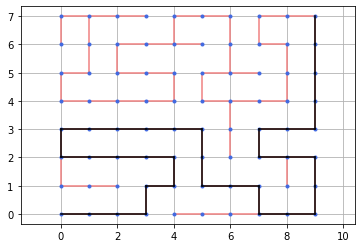
\includegraphics[width=\linewidth]{solution.png}
\caption{Solution d'un labyrinthe}
\end{marginfigure}
